\documentclass{article} 
\usepackage{geometry} 
\usepackage{longtable}
\usepackage{multicol} 
\usepackage[table]{xcolor}\geometry{a4paper, left=15mm, right=15mm, top=10mm} 
\usepackage[portuguese]{babel}
\usepackage[utf8]{inputenc}
\usepackage{graphicx}

\newcommand{\likert}{
\begin{figure}[h!]
\center
	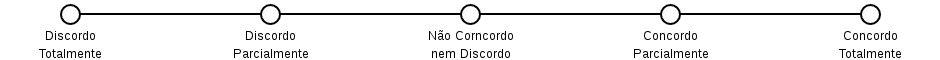
\includegraphics[width=0.8\textwidth]{Likert/likert.png} 
\end{figure}
}


%------------------------
\begin{document}


\begin{center}
\section*{Avaliação}
\end{center}


%\subsection*{Roteiro}
%% Jornada do usuário:
%Busca por palavras-chave $\rightarrow$ clique em um trecho $\rightarrow$ \{navegação pelo\}/\{análise do\} grupo do trecho.


\subsection*{Tarefas:}



\begin{itemize}
	\item Ler o texto introdutório à pesquisa;
	
	\item Analisar os resultados;
	\item Responder as questões.
\end{itemize}


\subsection*{Introdução}




Essa avaliação se refere a componentes de um sistema para consultas em atas de reunião. O objetivo dos sistema  é ajudar o usuário a fazer buscas por um assunto específico em uma coleção de atas de reunião. O Sistema deve receber uma consulta do usuário sobre um assunto e apresentar os trechos onde esse assunto é mencionado. As atas são documentos que não possuem um assunto principal, mas contém diversos assuntos registrados em um mesmo documento. Essa multiplicidade de assuntos das atas constitui um desafio para sistemas de consulta.

Inicialmente, o sistema analisa todas atas e divide o texto de cada ata em trechos que contêm um assunto principal e relativamente independente. Ou seja, os diversos assuntos tratados em uma ata são separados em trechos com um único assunto. Em seguida, utiliza-se técnicas de inteligência artificial para identificar trechos com assuntos relacionados e agrupá-los. Cada grupo contém trechos de atas diferentes mas com assuntos relacionados. Além disso, o sistema seleciona um conjunto de palavras que indicam o assunto do grupo. Assim, espera-se que o agrupamento de trechos com assuntos similares extraídos de diferentes documentos facilite a navegação e busca por assuntos na coleção de atas.

Para essa avaliação fez-se uma consulta ao sistema com os termos \textit{``compra de equipamentos''}. Três técnicas diferentes foram utilizadas para identificar trechos que tratam desse assunto e agrupá-los. Para cada um dos grupos apresentados, solicita-se que sejam respondidas algumas questões de forma a refletir a percepção do usuário quanto a qualidade dos resultados. 



\vspace{1cm}

Na imagem a seguir, é mostrada a tela principal do sistema com um campo para pesquisa na parte superior e abaixo os trechos pertencentes ao grupo selecionado. A esquerda estão os ícones seguidos de palavras que representam os grupos.


\begin{figure}[h!]
\center
	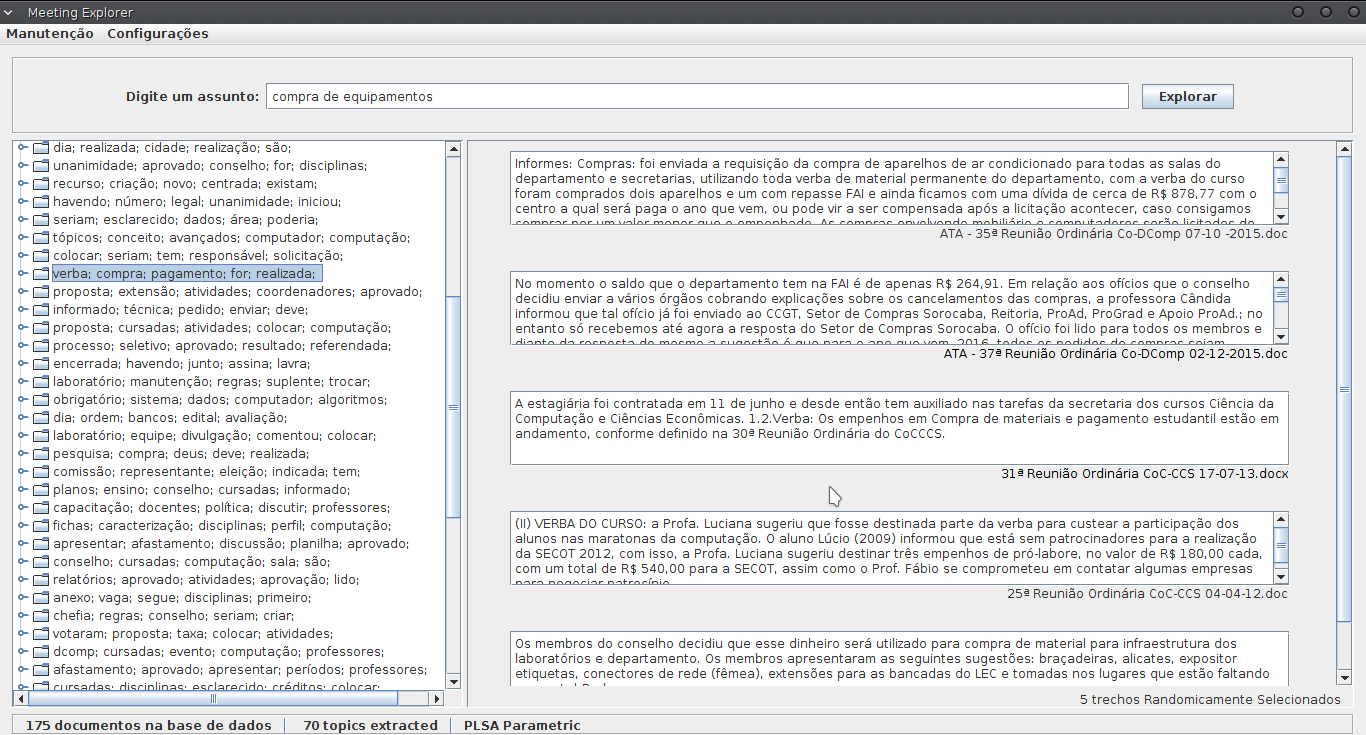
\includegraphics[width=1\textwidth]{prints/compra.png} 
\end{figure}







% --------------------


% --------------------

% Trata-se de um sistema para consultas em atas de reunião. O objetivo é ajudar o usuário a fazer buscas por um assunto específico em uma coleção de atas de reunião. O Sistema deve receber uma consulta do usuário sobre um assunto e apresentar os trechos onde esse assunto é mencionado. 

% Escolheu-se as atas por tratar-se de documentos que não possuem um assunto principal, mas contém diversos assuntos registrados em um mesmo documento. Essa multiplicidade de assuntos das atas constitui um desafio para sistemas de consulta e ao mesmo tempo motivou esse trabalho de mestrado.

% Para isso, visto a multiplicidade de assuntos uma mesma ata, o sistema inicialmente  analisa a coleção de atas e divide o texto de cada ata em trechos que contêm um assunto principal e relativamente independente. 
% Ou seja, os diversos assuntos tratados em uma ata são separados em trechos com um único assunto.
% Em seguida, utiliza-se técnicas de inteligência artificial para identificar trechos com assuntos relacionados e agrupá-los. Cada grupo contém trechos de atas diferentes mas com assuntos relacionados. Além disso, o sistema seleciona um conjunto de palavras descritoras que indicam o tópico do grupo. Nesse sistema, um grupo é formado por um conjunto de trechos e por um conjunto de palavras que o descreve.

% Assim, espera-se que o agrupamento de trechos com assuntos similares extraídos de diferentes documentos facilite a navegação e busca por assuntos na coleção de atas.

% Ao iniciar, o sistema apresenta os grupos anteriormente identificados os quais são representados por suas palavras descritoras. Ao selecionar um grupo, seus trechos são exibidos ao usuário para que possa verificar o que foi registrado sobre o assunto de cada grupo. 
% %
% O sistema também permite que o usuário faça consultas à coleção de atas por meio de um campo de pesquisa por palavras-chave. Nesse caso, o sistema  analisa as similaridades entre a consulta do usuário e os trechos extraídos das atas, bem como os grupos aos quais pertence. Então, apresenta os trechos ordenados pela relevância com a consulta do usuário. Para cada trecho é apresentado além do texto, um link para o arquivo original do qual foi extraído. Ao clicar sobre o texto de um trecho, seu grupo é destacado para que o usuário possa explorar outros trechos similares.


% Abaixo é mostrado a tela principal do sistema. A esquerda são apresentados os grupos com seus descritores e a direita os trechos atribuídos ao grupo selecionado. Acima está o campo para pesquisa.












% --> por que trechos? 

%Um trecho é representado por  texto  

%Com isso, espera-se que o agrupamento trechos de diferentes documentos, mas com assuntos similares, facilite a navegação e busca por assuntos na coleção de atas.


%Após realizar a busca, o sistema apresenta os trechos agrupados por tópicos, em que documentos com assuntos similares pertencem ao mesmo grupo. Ao selecionar um grupo, os trechos de atas são exibidos ao usuário.

%O sistema atribui um conjunto de palavras para cada grupo as quais servem para descrever o tópico do grupo.

%Cada grupo possui um conjunto de palavras 

%O sistema deve apresentar ao usuário os trechos de atas que melhor satisfazem a busca. 
 


%e documentos com assuntos diferentes ficam em gru



\newpage


\subsection*{Resultado de uma busca}
%\subsection*{Resultado de um agrupamento}

Segue abaixo o resultado de uma pesquisa no sistema à um conjunto de atas públicas obtidas pelo Departamento de Ciência da Computada da UFSCar campus Sorocaba. O resultado a ser analisado são os 10 primeiros trechos apresentados quando o usuário pesquisou pelos termos ``\textit{verba para compra de equipamentos}''.

\vspace{0.2 cm}


%\begin{longtable}{|p{17.6cm}|}
%\hline 
%\textbf{Descritores:}  planos, ensino, sistema, disciplinas, algoritmos\\ 
%\hline 
%\end{longtable} 

\begin{description}
\item[Pesquisa por: ] ``\textit{verba para compra de equipamentos}''
\end{description}

\noindent
\textbf{Trechos apresentados pelo sistema:}
\begin{longtable}{|p{0.2cm}|p{17cm}|}
\hline 
1 & 
(III.VIII) Foi deliberado que será elaborado um ofício, onde será relatada a realidade desse semestre, informando também que esse cenário será agravado nos próximos semestres (III.IX) A profª Katti solicita que seja evidenciado que para o próximo semestre, será necessário que um laboratório seja disponibilizado para os alunos da computação. \\ \hline 
2 &
Informes: A professora Sahudy informou que o ofício a respeito do processo de seleção do PIBIC será enviado, no entanto o tom do ofício foi suavizado, informou também que tem um valor em auxílio estudante que precisará liquidar ainda este ano, pois provavelmente ele não virará o ano por ser de 2015, sendo assim está aceitando sugestões para gastos do referido dinheiro com apoio a projetos de disciplinas no valor máximo de até 800 reais e o que sobrar será enviado como ajuda custos para SeCoT 2017.
 \\ \hline 
3 &
Informes:. (I) RESPOSTA AO OFÍCIO DE COMPRAS. (I.I) A professora Sahudy informou que somente o setor de compras/Sorocaba respondeu ao ofício 038/2015, os demais não se manifestaram, e ainda devolveram os ofícios, pois entendem que a responsabilidade da resposta do ofício em questão é de competência do setor de compras Sorocaba. Os professores não aceitaram tal justificativa e solicitaram que os ofícios sejam enviados novamente. O pedido foi aceito. (II) INFORME SOBRE COMPRAS DE MATERIAL PERMANENTE. (II.I) Foi informado que serão atendidos as prioridades 1 e 2 da tabela de preferência.
 \\ \hline 
4 &
Informes:. A professora Sahudy informou que no semestre anterior foi aprovado em reunião um dia específico para a manutenção dos laboratórios e pediu para o técnico não marcar médico e respeitar os horários nos dias da manutenção e também fazer um relatório dos problemas encontrados.
 \\ \hline 
5 &
(II.I) A professora Sahudy informou que gastou R\$ 3584,65 com material de informática, e que a cópia de prestação de contas está na secretaria do DComp, e informou também que a verba RTI de 2015 também já foi liberada, porém só será utilizada quando terminar a prestação de contas do CCTS referente a 2014. (III) REDISTRIBUIÇÃO DO TÉCNICO THIAGO. (III.I) A professora Sahudy informou que o técnico Thiago André Pereira Leite, solicitou redistribuição para o Instituto Federal de São Paulo e que ela aprovou ad referendum o pedido do mesmo, não esquecendo que tal redistribuição tem como condição a permuta de vagas.
 \\ \hline 
6 &
Informes: O Prof. Gustavo informou que os pedidos de compra estão sendo realizados no novo sistema como planejado. Também informou que o ar-condicionado do LEC foi instalado. 
\\ \hline 
7 &
(II) Informou também sobre o atraso da verba 18 PROAP para 2015, que segundo informações da Pró-Reitora deverá ser liberado ao final 19 de fevereiro;
Informes:.A professora Cândida informou que a licitação de compra dos aparelhos de ar condicionado deu certo e que em breve os mesmos serão instalados; também informou que a atividade de extensão (Desenvolvimento em Nuvem;
 \\ \hline 
8 &
3.4 Verba do curso: foi deliberado que a verba da coordenação do curso será destinada para compra de ar condicionado e para a organização do Workshop de Intercâmbio de Experiências em Computação que está sob responsabilidade do prof. José de Oliveira Guimarães.
 \\ \hline 
9 &
(IV) PATRIMÔNIOS (TERMOS DE RESPONSABILIDADE). (IV.I) A professora Sahudy esclareceu que foi enviado um e-mail ontem com as duas opções que seriam discutidas hoje e colocada em votação. 1) O chefe do departamento ficaria responsável pelos bens comuns e cada um seria responsável pelo que tem na sala. 2) O chefe ficaria responsável por todos os patrimônios. Foi colocado em votação, sendo 5 votos para primeira opção e 2 para a segunda. Sobre os equipamentos de doações vamos verificar em que nome tem saído os termos de responsabilidade.
 \\ \hline 
10 &
Informes: Compras: foi enviada a requisição da compra de aparelhos de ar condicionado para todas as salas do departamento e secretarias, utilizando toda verba de material permanente do departamento, com a verba do curso foram comprados dois aparelhos e um com repasse FAI e ainda ficamos com uma dívida de cerca de R\$ 878,77 com o centro a qual será paga o ano que vem, ou pode vir a ser compensada após a licitação acontecer, caso consigamos comprar por um valor menor que o empenhado. As compras envolvendo mobiliário e computadores serão licitados de formas diferentes, será realizado um pedido para toda a universidade e serão comprados via ata, maiores informações de gastos verificar planilha anexa.

 \\ \hline 

\end{longtable} 



\newpage

\subsection*{Questões}

Com base na análise do resultado apresentado, por favor qual sua concordância com a afirmações a seguir:

\begin{enumerate}

\item A ordem na qual os trechos são apresentados está de acordo com a relevância ao assunto pesquisado.
\likert

\item Os trechos apresentados satisfazem/respondem bem à consulta.
\likert

\item Os trechos apresentados estão bem relacionados à consulta.
\likert

\item A leitura de um trecho é suficiente para entender o assunto desse trecho.
\likert

\item Os trechos apresentados são suficientes para entender o tópico.
\likert

\end{enumerate}





%\begin{multicols}{5}
%
%\begin{itemize}
%\item Nada
%\item Pouco
%\item Razoável
%\item Bom
%\item Excelente
%\end{itemize}
%
%\end{multicols}
%
%\begin{multicols}{5}
%
%\begin{itemize}
%\item Discordo Totalmente
%\item Discordo Parcialmente
%\item Não Concordo nem Discordo
%\item Concordo Parcialmente
%\item Concordo Totalmente
%\end{itemize}
%



















\newpage


\subsection*{Resultado de uma consulta}
%\subsection*{Resultado de um agrupamento}

%Após realizar a busca por palavras chave, o usuário selecionou o grupo ao qual pertence o trecho 5 dos resultados anteriores.
%Abaixo estão relacionados os 10 primeiros trechos que o sistema apresentou após essa ação bem como os descritores desse grupo.


Segue abaixo o resultado de uma pesquisa no sistema à um conjunto de atas públicas obtidas pelo Departamento de Ciência da Computação da UFSCar campus Sorocaba. O resultado a ser analisado são os 10 primeiros trechos apresentados quando o usuário pesquisou pelos termos ``\textit{defesa de dissertação}''.

\vspace{0.5 cm}


% é possível analisar o grupo ao qual cada trecho pertence para encontrar outros resultados similares. 



%\begin{longtable}{|p{17.6cm}|}
%\hline 
%\textbf{Descritores:}  planos, ensino, sistema, disciplinas, algoritmos\\ 
%\hline 
%\end{longtable} 

\begin{description}
\item[Palavras descritoras: ] orientada, meses, defesa, prazo, dissertação
\end{description}


\noindent
\textbf{Trechos apresentados pelo sistema:}
\begin{longtable}{|p{17.5cm}|}
\hline 
%1 & 
Também foi discutida a situação de alunos que recebem a bolsa no decorrer do curso e apresentam o exame de defesa antes do término do prazo da bolsa. A duração da bolsa oferecida pela CAPES é de 24 meses e foi apresentada a proposta do aluno continuar com a bolsa caso solicite prorrogação do prazo de defesa da dissertação, desde que mantenha os requisitos descritos na norma 5 e não tenha nenhum aluno na lista de espera do ranking de bolsas elaborado pela Comissão de Bolsas de Estudos do PPGCCS. Foi decidido retirar os seguintes requisitos da norma 5: 1. b) Não ter completado 12 (doze) meses corridos a contar da data de sua primeira matrícula no curso de Mestrado, exceto no caso de renovação. 3. d) ultrapassar 24 (vinte e quatro) meses no Programa, ou 3. e) não tiver cumprido a Norma 6 sobre obrigatoriedade de solicitação de Bolsa FAPESP.

 \\ \hline 
%2 &
(II) Aprovado o pedido de prorrogação de prazo para defesa de dissertação do aluno Daniel Ianegitz Vieira por mais 06 meses com prazo final para fevereiro de 2016. A partir de agora o formulário para solicitação de prorrogação de prazo para defesa de dissertação possui a opção de prorrogar a bolsa de estudos: No último mês de vigência da bolsa de estudos, será consultada a lista de espera por bolsas do PPGCCS. A solicitação de prorrogação de bolsa só será analisada caso não existam candidatos na fila de espera e se a vigência da bolsa não tiver atingido 24 meses. Neste caso, se a prorrogação for atendida, o novo prazo de vigência da bolsa será estendido para coincidir com a data prevista da defesa ou até que se complete 24 meses de bolsa (o que ocorrer primeiro);
 \\ \hline 
%3 &
(V) Homologado o Relatório de Defesa de Dissertação da aluna Talita dos Reis Lopes Berbel, orientada pela Profa. Dra. Sahudy Montenegro González e do aluno Tiago Vanderlei de Arruda, orientado pela Profa. Dra. Tiemi Christine Sakata; (VI) Aprovado o pedido de agendamento de exame de defesa de dissertação do aluno Marcus Vinicius Sandri, orientado pelo Prof. Dr. Fábio Luciano Verdi com participação do Prof. Dr. Christian Rodolfo Esteve Rothemberg da UNICAMP e da Profa. Dra. Yeda Regina Venturini como membros da banca examinadora;
 \\ \hline 
%4 &
(III) aprovado o pedido de prorrogação de prazo para defesa de dissertação do aluno Tiago Pasqualini da Silva, orientado pelo Prof. Dr. Tiago Agostinho de Almeida por mais 06 meses com prazo final para setembro de 2015;
 \\ \hline 
%5 &
(III) Homologados os relatórios de defesa de dissertação dos alunos Anderson Parra de Paula, Marcus Vinícius Sandri, Rogério Colpani e Wilton Moreira Ferraz Junior.

 \\ \hline 
%6 &
%(I.IV) A Profa. Dra. Katti Faceli apresenta a disciplina Inteligência Artificial.
% \\ \hline 
%7 &
%(I.VII) Prof. Dr. Siovani Cintra Felipussi apresenta as disciplinas Noções Básicas de Economia, Gestão de Pequenas Empresas, Probabilidade e Estatística e Geometria Analítica e Álgebra Linear.
% \\ \hline 
%8 &
%(I.VIII) Após discussão sobre os objetivos, ementas, distribuição de créditos e requisitos, as fichas de caracterização para o perfil 3, a serem oferecidas no primeiro período letivo de 2009, foram aprovadas como segue: Disciplina CR Teo Lab CH Introdução aos Sistemas de Informação 04 04 00 60 Algoritmos e Complexidade 04 03 01 60 Inteligência Artificial 04 03 01 60 Arquitetura e Organização de Computadores 04 04 00 60 Estrutura de Dados 2 04 03 01 60 Noções Básicas de Economia 02 02 00 30 Gestão de Pequenas Empresas 02 02 00 30 Probabilidade e Estatística 04 04 00 60 Geometria Analítica e Álgebra Linear 04 04 00 60 A disciplina Geometria Analítica e Álgebra Linear teve sua ficha de caracterização aprovada com ressalva.
% \\ \hline 
%9 &
%Após discussão o espelhamento é aprovado por unanimidade como segue: Disciplina CR Teo Lab CH Algoritmos e Programação de Computadores 08 04 04 120 Cálculo Diferencial e Integral 1 04 03 01 60 Física para Computação 04 03 01 60 Geometria Analítica e Álgebra Linear 04 04 00 60 Lógica para Computação 04 03 01 60 (III) DISCUSSÃO SOBRE O REAPROVEITAMENTO DE VAGAS: (II.I) O presidente discorre brevemente sobre a distribuição de vagas já discutida em reunião anterior.
% \\ \hline 
%10 &
%A avaliação dos planos de ensino de cada disciplina oferecida no curso de Ciência da Computação foi atribuída para cada professor, as avaliações foram devidamente realizadas e os pareceres efetuados pelos respectivos professores bem como os planos de ensino na íntegra foram submetidos à avaliação do conselho que decidiu por unanimidade.
% \\ \hline 

\end{longtable} 



\newpage

\subsection*{Questões}


Com base na analise do resultado apresentado, por favor qual sua concordância com a afirmações a seguir:


%responda as seguintes questões:



\begin{enumerate}

\item A observação do grupo permite encontrar outros trechos relacionados ao assunto.
\likert

\item É possível identificar claramente os assuntos do grupo com bases nos descritores.
\likert

\item É possível encontrar trechos relacionados pelos agrupamento dos trechos.
\likert

\item Os descritores dos grupos são bons representantes do assunto dos trechos?
\likert

\item Os trechos apresentados são suficientes para entender o tópico.
\likert

\item Os trechos apresentados estão bem relacionados entre si.
\likert

\item Os trechos apresentados estão bem relacionados os descritores.
\likert

\item Ao analisar outros trechos do mesmo grupo, e possível obter informações extras, não contidas no trecho inicial.
\likert

%\item A navegação pelos tópicos ajuda a conduzir o usuário para o documento desejado.
%\likert

\end{enumerate}







%\begin{multicols}{5}
%
%\begin{itemize}
%\item Nada
%\item Pouco
%\item Razoável
%\item Bom
%\item Excelente
%\end{itemize}
%
%\end{multicols}
%
%\begin{multicols}{5}
%
%\begin{itemize}
%\item Discordo Totalmente
%\item Discordo Parcialmente
%\item Não Concordo nem Discordo
%\item Concordo Parcialmente
%\item Concordo Totalmente
%\end{itemize}
%



















\end{document}




